\documentclass[Total.tex]{subfiles}

\begin{document}
	\chapter{Fundamentals}
		\section{Topology of Mappings}
			\subsection{CW Decompsoition}
				Given in other parts of topology. 
		\section{Degree of Maps}
			\subsection{Orientation}
				\subsubsection{Unbounded Manifold}
				\begin{Def}
					\begin{itemize}
						\item The orientation of an  Euclidean $n$-space is given by the basis with positive determinant. i.e. $det(v_1,\dots,v_n)>0$;
						\item An oriented atlas is a family of charts
						\begin{gather*}
							\mathcal{A}:=\{(U_\alpha,x_\alpha)\}_{\alpha\in I}
						\end{gather*}
						
						such that
						\begin{gather*}
							det(x_\alpha\circ x_\beta^{-1})>0
						\end{gather*}
						\item An oriemtation of a real-manifold is given by a frame
						\begin{gather*}
							\theta=(\theta^1,\dots,\theta^n)
						\end{gather*}
						
						where for every coordinate chart (in oriented atlas) $\varphi=(\varphi_1,\dots,\varphi_n):U\rightarrow V\subseteq \RR^n$, 
						\begin{gather*}
							内容...
						\end{gather*}
						\item Product: Given two oriented manifolds $(M,\omega),(N,\theta)$
						\begin{gather*}
							(
							M\times N,\omega\oplus \theta)
						\end{gather*}
					\end{itemize}
				\end{Def}
				
				\subsubsection{Bounded Manifold}
				
				\subsubsection{Submanifold}
			\subsection{Degree}
				\begin{lemma}
					(Orientation induced by Arc)Let 
					\begin{itemize}
						\item $(W,\omega)$ be an oriented $\partial$-manifold;
						\item $K\subseteq W$ is an embedded arc which is transverse to $\partial W$ at its endpoint $u,v\in \partial W$
					\end{itemize}
					
					Then, consider the quotient orientation $(W/K,\omega/\kappa)$, then
					\begin{gather*}
						\omega_u/\kappa_u=(\partial\omega)_u\Leftrightarrow \omega_v/\kappa_v=-(\partial \omega)_v
					\end{gather*}
				\end{lemma}
				\begin{proof}
					This is equivalent to: Inward and outward. 
					
					And the tranverse at $u,v$ in $\partial W$ means
					\begin{gather*}
						T_u(\partial W)\oplus T_u(K)=T_u W
					\end{gather*} 
					
					And the orientation of $W$ is specified by the direction $\pm 1$ of arc curve.
				\end{proof}
				
				A concrete example is an area on plane:
				\begin{figure}[htbp]
					\centering
					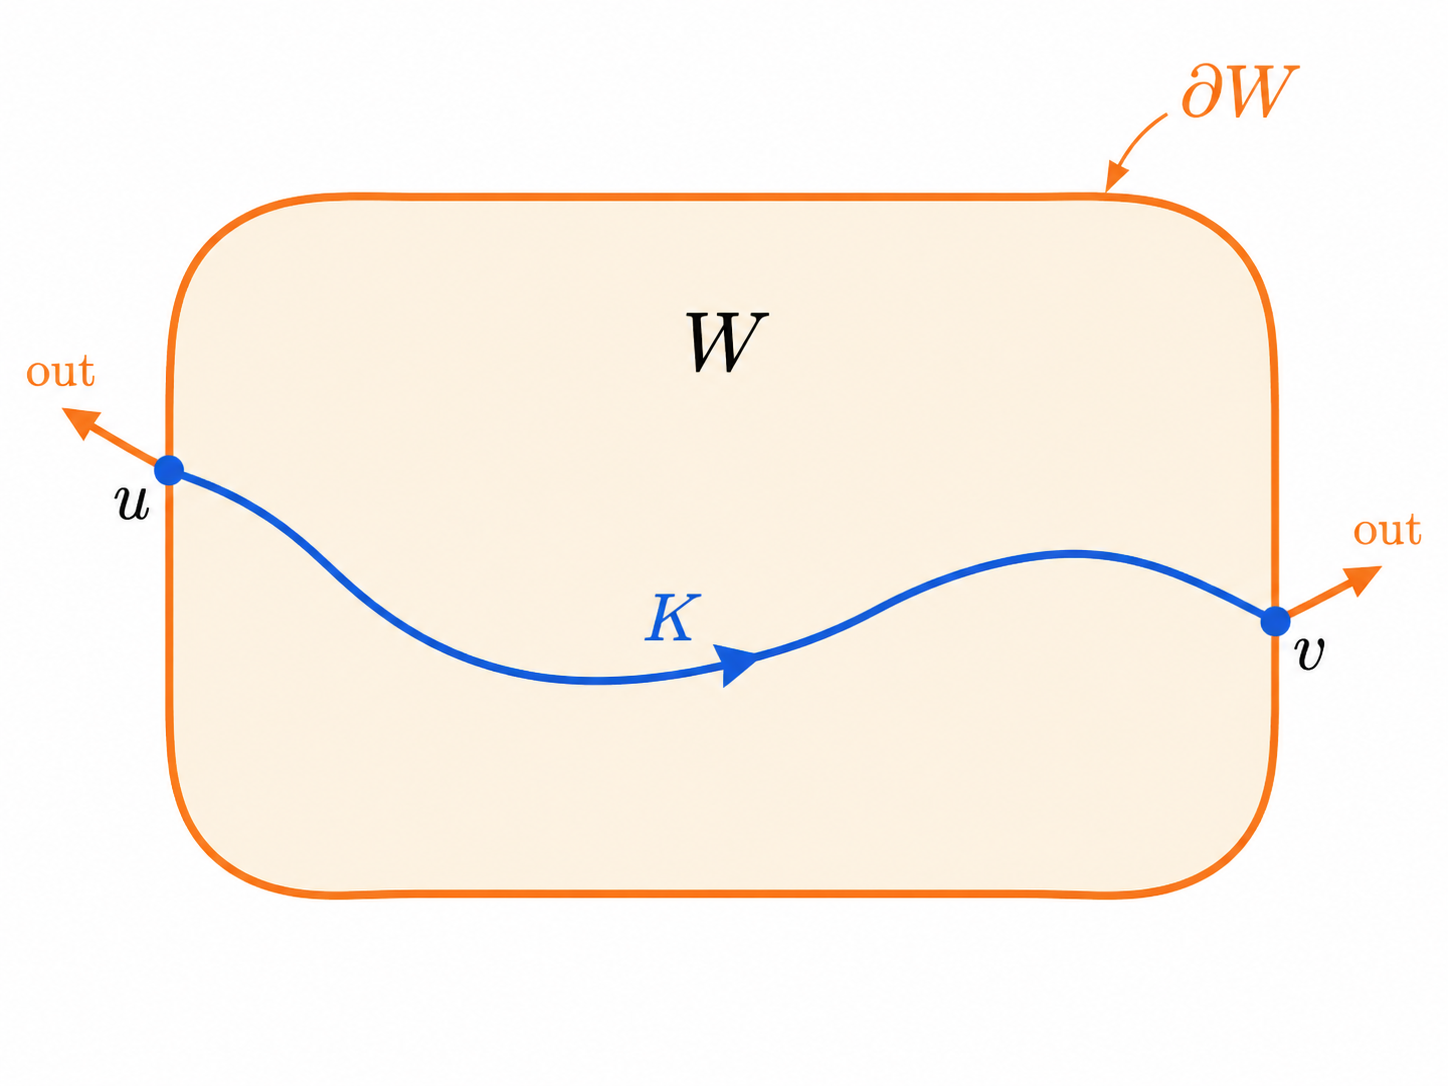
\includegraphics[scale=0.1]{DT-01.png}
				\end{figure}
				\begin{Def}
					Let:
					\begin{itemize}
						\item $(M,\omega),(N,\theta)$ are \underline{compact oriented} smooth manifold;
						
						Same dimension $dim(M)=dim(N)$;
						
						$(N,\theta)$ is connected; 
						\item $f\in C^1(M,N)$;
						\item $x$ is a regular point of $f$, i.e. $df_x$ is surjective. Equivalently, $df_x$ is linear isomorphism;
					\end{itemize}
					
					Then, define: For $x\in M,y=f(x)$: $x$ has \textbf{positive type} if the isomorphism $T_xf:T_x M\rightarrow T_{f(x)} N=T_y N$ preserves orientation
					\begin{itemize}
						\item $deg_x(f):=1$, if positive;
						\item $deg_x(f):=-1$, is negative;
					\end{itemize}
					
					Finally,
					\begin{gather*}
						deg(f,y):=\sum_{x\in f^{-1}(y)} deg_x f:=\sum_{x\in f^{-1}(y)} deg_x(f)
					\end{gather*}
				\end{Def}
				
				The sum is well-defined, because: $N$ is compact
				
				\textbf{Remark} In principle, we could have weaker requirement for definition of degree:
				\begin{itemize}
					\item $M$ is compact;or
					\item $f$ is proper.
				\end{itemize}
				
				Then, $\{y\}\subseteq N$ is compact, thus $f^{-1}(y)$ is compact. Then, by inverse function theorem, there exists a local diffeomorphism(thus injective)
				\begin{gather*}
					f|U_p:U_p\rightarrow f(U_p)\qquad f(p)=y\qquad 
				\end{gather*}
				
				Then, $f^{-1}(p)$ is discrete. Finally, by compactness, is finite.
				
				\begin{proposition}
					If $M$ is compact, then
					\begin{gather*}
						deg(f)=\sum deg(f|M)
					\end{gather*}
				\end{proposition}
				\begin{proof}
					Notice, by compactness, $M=\sqcup M_i$, finite coproduct.
				\end{proof}
				
				\subsection{Degree as Homotopic Invariance}
				
				\begin{proposition}
					Let: 
					\begin{itemize}
						\item $W$ be a compact oriented manifold of dimension $n+1$;
						\item $N$ be a compact oriented $n$-manifold without boundary;
						\item $h:W\rightarrow N$ be $C^\infty$ map;
						\item $y\in N$ be a regular value for both $h$ and $h|\partial W$; i.e.
						\begin{center}
							$dh_p:T_p W\rightarrow T_{y}N$ is surjective, $p\in h^{-1}(y)$\qquad $dh_p|_{T_p(\partial W)}:T_p(\partial W)\rightarrow T_p N$ is surjective. 
						\end{center}
					\end{itemize}
					
					Then,
					\begin{gather*}
						deg(h|\partial W,y)=0
					\end{gather*}
				\end{proposition}
				\begin{proof}
					Notice $y$ is a regular value, then $h^{-1}(y)$ is a compact $1$-dimensional submanifold of $W$: Compacatness by $\{y\}$, and $1$-dimensional submanifold by property of regular element. (By regular value set theorem, and is embedding), with boundary $(h|\partial W)^{-1}(y)$. 
					
					Then, $f=h|\partial W$:
					\begin{gather*}
						deg(f,y)=\sum_{x\in f^{-1}(y)} deg_x(f)=\sum_{x\in f^{-1}(y)\cap  \partial M} deg_x(f)
					\end{gather*}
					
					For $L=h^{-1}(y)$, $\partial L=L\cap \partial W$. With compactness, component $x\in K\cong I$ or $x\in K\cong S^1$. But $\partial S^1=\emptyset$, so $K\cong I$. There exists another endpoint $x'\in K\subseteq L$. 
					
					Thus, 
					\begin{gather*}
						\sum_{x\in f^{-1}(y)\cap \partial M} deg_x(f)=0
					\end{gather*}
					
					We will not counting twice because of the component decomposition. 
				\end{proof}
				
				\begin{corollary}
					Let $(M,\omega),(N,\theta)$ be compact, oriented $n$-manifold, $\partial M=\partial N=\emptyset$. 
					
					$N$ is connected, and $f\simeq_{h} g$ be $C^\infty$ maps, having a common regular value $y\in N$, then
					\begin{gather*}
						deg(f,y)=deg(g,y)
					\end{gather*}
				\end{corollary}
				\begin{proof}
					Now instead of $h$, we use the homotopy $F:M\times I\rightarrow N$;
					
					And the boundary $\partial(M\times I)=(\partial M\times 0,\omega)\cup (\partial M\times 1,-\omega)$. We obtain that
					\begin{gather*}
						0=deg(F)=deg(f,y;\omega,\theta)+deg(g,y;-\omega,\theta)=deg(f,y;\omega,\theta)-deg(g,y;\omega,\theta)
					\end{gather*}
				\end{proof}	
				
			\subsection{Degree at Different Regular Value}
			
			\subsection{Approxiamation}
			
			\subsection{mod 2 Degree: Homotopic Invariance}
				Notice $deg_x(f)$ must be $\pm 1$, it is convenient to observe their value mod $2$: 
				
				Firstly, we could calculating the degree by apporoxiamation: $f\simeq g,g\in C^\infty(M,N)$
				\begin{gather*}
					deg(f)=deg(g,z)
				\end{gather*}
			
				\begin{Def}
					Suppose:
					\begin{itemize}
						\item $M,N$ are not oriented(even nonorientable); 
						\item $f:M\rightarrow N$ continuous;
						\item $g:M\rightarrow N$ homotopic to $f$; $g\in C^\infty(M,N)$;
					\end{itemize}
					
					Then, $deg_2(g,z):=\#g^{-1}(z)\mod 2$. 
				\end{Def}
				
				By our discussion of $n+1$ manifold in $n$ manifold, the regular points have paring, thus $deg_2(g,z)$ is independent of choice of $z$ and orientation. 
				
				\subsubsection{Homology with Coefficient $\ZZ/2\ZZ$}
				
				\subsubsection{Oriented and Nonorientable Manifolds}
				\subsubsection{Calculating of Fundamental Groups}
				\subsubsection{Application: Contractibility}
				\subsubsection{Application: Surjectivity}
				\subsubsection{Example: Klein Bottle}
		\section{Intersection Numbers and Euler Characteristics}
			\subsection{Intersection Number}
				\begin{Def}
					Let: 
					\begin{itemize}
						\item $W$ be an oriented manifold of dimension $m+n$;
						\item $N\subseteq W$ a closed oriented submanifold of dimension $n$;
						\item $M$ be a compact oriented $m$-manifold;
						\item $\partial M=\partial N=\emptyset$;
						\item $f\in C^\infty(M,W)$, transverse to $N$;
					\end{itemize}
					
					Then, consider the following composition
					\begin{gather*}
						T_xM\stackrel{Tf_x}{\rightarrow} T_{f(x)}W\rightarrow T_{f(x)}W/T_{f(x)}N
					\end{gather*}
					
					If it is orientation-preserving, then $\#_x(f,N)=1$; If orientation-reversing, then $\#_x(f,N)=-1$, and 
					\begin{gather*}
						\#(f,N)=\sum \#_x (f,N)
					\end{gather*}
				\end{Def}
				
				\begin{theorem}
					(Intersection Number as Homotopic Invariance)
				\end{theorem}
				\begin{proof}
					内容...
				\end{proof}
				
				\subsection{Euler Number}
				
				\subsection{Euler Characteristics}
				
		
		\section{Hopf's Degree Theorem}
			Recall:
			\begin{lemma}
				Every smooth oriented $n$-manifold could have a Riemann metric.
			\end{lemma}
			\begin{proof}
				Given in Riemann surface.
			\end{proof}
			\begin{theorem}
				(Hopf's Degree Theorem) Let: $M$ be a connected oriented closed smooth manifold of dimension $n\geq 1$, then the degree defines a bijection
				\begin{gather*}
					deg:[M,S^n]\rightarrow \ZZ
				\end{gather*}
				
				where $[-,-]$ for the homotopy class. 
			\end{theorem}
			\begin{proof}
				内容...
			\end{proof}
			
			\begin{corollary}
				
			\end{corollary}
			\begin{proof}
				内容...
			\end{proof}
			
		\section{Pontrjagin-Thom Construction}
		
	
	\chapter{Morse Theory}
		We will introduce this in 'Morse theory and Floer theory';
	\chapter{Cobordism}
		This is a relative large topic. 
	\chapter{Isotopy}
	
	\chapter{Surfaces}
\end{document}